\documentclass[multi=tikzpicture,border=10pt]{standalone}
\usepackage{tikz}
\usepackage[compat=1.1.0]{tikz-feynman}

% ===== 字体：需要 XeLaTeX =====
\usepackage{fontspec}
\usepackage{xeCJK}
\usepackage{unicode-math}

% 正文
\setmainfont{Libertinus Serif}

% 数学
\setmathfont{Latin Modern Math}
\tikzset{
  source dot/.style={
    circle, fill=black, draw=black, inner sep=0pt, minimum size=5.5mm
  },
  blob/.style={
    circle, draw=black, thick, fill=white, inner sep=0pt, minimum size=12mm
  },
  blob with insertion/.style={
    circle, draw=black, thick, fill=white, inner sep=0pt, minimum size=12mm,
    path picture={
      \draw[black, thick]
      (path picture bounding box.north) -- (path picture bounding box.south);
    }
  }
}
\begin{document}

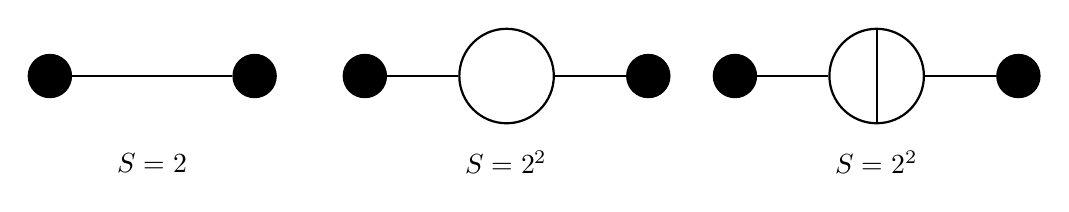
\begin{tikzpicture}


% 第一行第1个：黑点-线段-黑点
\begin{scope}[shift={(0,0)}]
  \node[source dot] (aL) at (-1.3,0) {};
  \node[source dot] (aR) at ( 1.3,0) {};
  \begin{feynman}
    \diagram*{
      (aL) -- [draw=black, thick] (aR),
    };
  \end{feynman}
  \node at (0,-1.1) {$S=2$};
\end{scope}

% 第一行第2个：黑点-圆blob-黑点
\begin{scope}[shift={(4.5,0)}]
  \node[source dot] (bL) at (-1.8,0) {};
  \node[blob]       (bM) at ( 0.0,0) {};
  \node[source dot] (bR) at ( 1.8,0) {};
  \begin{feynman}
    \diagram*{
      (bL) -- [draw=black, thick] (bM),
      (bM) -- [draw=black, thick] (bR),
    };
  \end{feynman}
  \node at (0,-1.1) {$S=2^2$};
\end{scope}

% 第一行第3个：黑点-带插入线的圆blob-黑点
\begin{scope}[shift={(9.2,0)}]
  \node[source dot]           (cL) at (-1.8,0) {};
  \node[blob with insertion]  (cM) at ( 0.0,0) {};
  \node[source dot]           (cR) at ( 1.8,0) {};
  \begin{feynman}
    \diagram*{
      (cL) -- [draw=black, thick] (cM),
      (cM) -- [draw=black, thick] (cR),
    };
  \end{feynman}
  \node at (0,-1.1) {$S=2^2$};
\end{scope}

\end{tikzpicture}


\newpage
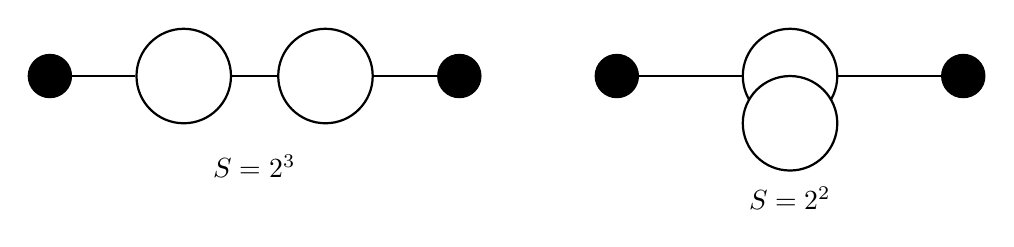
\begin{tikzpicture}
    % ------------------------------------------------
% 第二行第1个：黑点-圆blob-圆blob-黑点
% ------------------------------------------------
\begin{scope}[shift={(2.6,-3.2)}]
  \node[source dot] (dL) at (-2.6,0) {};
  \node[blob]       (d1) at (-0.9,0) {};
  \node[blob]       (d2) at ( 0.9,0) {};
  \node[source dot] (dR) at ( 2.6,0) {};

  \begin{feynman}
    \diagram*{
      (dL) -- [draw=black, thick] (d1),
      (d1) -- [draw=black, thick] (d2),
      (d2) -- [draw=black, thick] (dR),
    };
  \end{feynman}
  \node at (0,-1.15) {$S=2^3$};
\end{scope}

% ------------------------------------------------
% 第二行第2个：上方blob接两外源，下方再接一个blob
% ------------------------------------------------
\begin{scope}[shift={(9.4,-3.2)}]
  \node[source dot] (eL) at (-2.2,0) {};
  \node[blob]       (eT) at ( 0.0,0) {};
  \node[source dot] (eR) at ( 2.2,0) {};
  \node[blob]       (eB) at ( 0.0,-0.60) {};

  \begin{feynman}
    \diagram*{
      (eL) -- [draw=black, thick] (eT),
      (eT) -- [draw=black, thick] (eR),
      %(eT) -- [draw=black, thick] (eB),
    };
  \end{feynman}
  \node at (0,-1.55) {$S=2^2$};
\end{scope}
\end{tikzpicture}



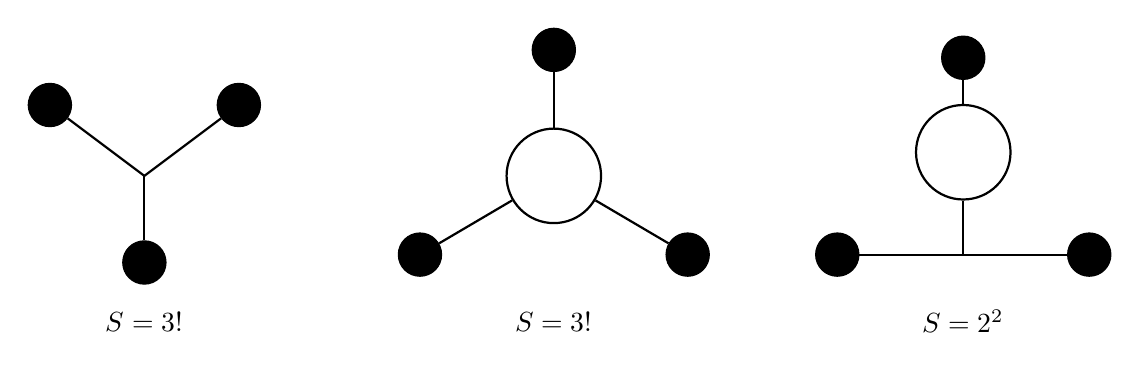
\begin{tikzpicture}

% 第三行左：Y 形三叉（全黑点）
\begin{scope}[shift={(0,0)}]
  \node[source dot] (a1) at (-1.2, 0.9) {};
  \node[source dot] (a2) at ( 1.2, 0.9) {};
  \node[source dot] (a3) at ( 0.0,-1.1) {};
  \coordinate (ac) at (0,0);

  \draw[thick] (ac) -- (a1);
  \draw[thick] (ac) -- (a2);
  \draw[thick] (ac) -- (a3);
   \node at (0,-1.85) {$S=3!$};
\end{scope}

% 第三行中：中心 blob + 三条腿
\begin{scope}[shift={(5.2,0)}]
  \node[blob]       (b0) at (0,0) {};
  \node[source dot] (b1) at ( 0.0, 1.6) {};
  \node[source dot] (b2) at (-1.7,-1.0) {};
  \node[source dot] (b3) at ( 1.7,-1.0) {};

  \draw[thick] (b0) -- (b1);
  \draw[thick] (b0) -- (b2);
  \draw[thick] (b0) -- (b3);
  \node at (0,-1.85) {$S=3!$};
\end{scope}

% 第三行右：竖直 blob，下方水平双外源
\begin{scope}[shift={(10.4,0)}]
  \node[blob]       (c0) at (0,0.3) {};
  \node[source dot] (c1) at (0,1.5) {};
  \node[source dot] (c2) at (-1.6,-1.0) {};
  \node[source dot] (c3) at ( 1.6,-1.0) {};
  \coordinate (cb) at (0,-1.0);

  \draw[thick] (c1) -- (c0);
  \draw[thick] (c0) -- (cb);
  \draw[thick] (c2) -- (cb) -- (c3);
  \node at (0,-1.85) {$S=2^2$};
\end{scope}

\end{tikzpicture}





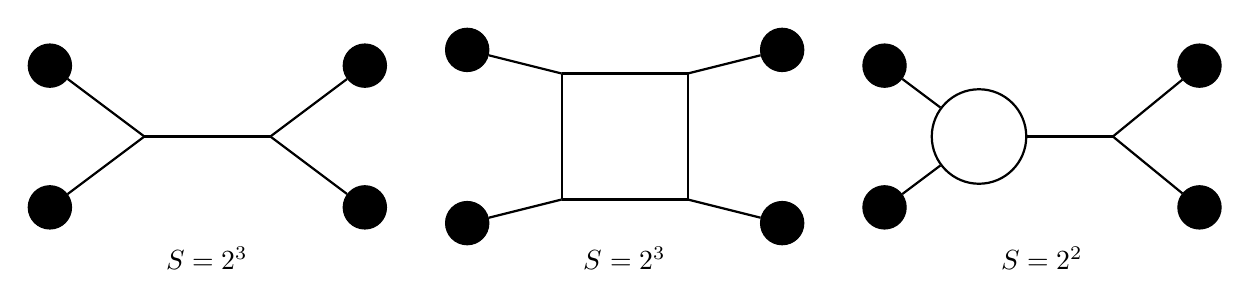
\begin{tikzpicture}
    % ------------------------------------------------
% 第4行第1个：两个三价顶点相连（4个外源）
% ------------------------------------------------
\begin{scope}[shift={(2.6,-7.0)}]
  \node[source dot] (fLT) at (-2.0, 0.9) {};
  \node[source dot] (fLB) at (-2.0,-0.9) {};
  \node[source dot] (fRT) at ( 2.0, 0.9) {};
  \node[source dot] (fRB) at ( 2.0,-0.9) {};

  \begin{feynman}
    \vertex (fL) at (-0.8,0);
    \vertex (fR) at ( 0.8,0);
    \diagram*{
      (fLT) -- [draw=black, thick] (fL),
      (fLB) -- [draw=black, thick] (fL),
      (fL)  -- [draw=black, thick] (fR),
      (fR)  -- [draw=black, thick] (fRT),
      (fR)  -- [draw=black, thick] (fRB),
    };
  \end{feynman}
  \node at (0,-1.55) {$S=2^3$};
\end{scope}

% ------------------------------------------------
% 第三行第2个：四边形 loop（四个外源接四角）
% ------------------------------------------------
\begin{scope}[shift={(7.9,-7.0)}]
  \node[source dot] (gLT) at (-2.0, 1.1) {};
  \node[source dot] (gRT) at ( 2.0, 1.1) {};
  \node[source dot] (gRB) at ( 2.0,-1.1) {};
  \node[source dot] (gLB) at (-2.0,-1.1) {};

  \begin{feynman}
    \vertex (g1) at (-0.8, 0.8);
    \vertex (g2) at ( 0.8, 0.8);
    \vertex (g3) at ( 0.8,-0.8);
    \vertex (g4) at (-0.8,-0.8);
    \diagram*{
      (g1) -- [draw=black, thick] (g2),
      (g2) -- [draw=black, thick] (g3),
      (g3) -- [draw=black, thick] (g4),
      (g4) -- [draw=black, thick] (g1),

      (gLT) -- [draw=black, thick] (g1),
      (gRT) -- [draw=black, thick] (g2),
      (gRB) -- [draw=black, thick] (g3),
      (gLB) -- [draw=black, thick] (g4),
    };
  \end{feynman}
  \node at (0,-1.55) {$S=2^3$};
\end{scope}

% ------------------------------------------------
% 第三行第3个：左侧blob + 右侧三价顶点（4个外源）
% ------------------------------------------------
\begin{scope}[shift={(13.2,-7.0)}]
  \node[source dot] (hLT) at (-2.0, 0.9) {};
  \node[source dot] (hLB) at (-2.0,-0.9) {};
  \node[blob]       (hB)  at (-0.8,0) {};
  \node[source dot] (hRT) at ( 2.0, 0.9) {};
  \node[source dot] (hRB) at ( 2.0,-0.9) {};

  \begin{feynman}
    \vertex (hR) at (0.9,0);
    \diagram*{
      (hLT) -- [draw=black, thick] (hB),
      (hLB) -- [draw=black, thick] (hB),
      (hB)  -- [draw=black, thick] (hR),
      (hR)  -- [draw=black, thick] (hRT),
      (hR)  -- [draw=black, thick] (hRB),
    };
  \end{feynman}
  \node at (0,-1.55) {$S=2^2$};
\end{scope}
\end{tikzpicture}


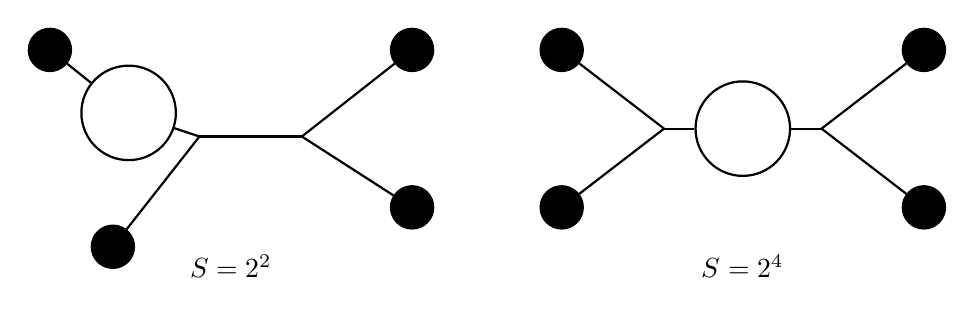
\begin{tikzpicture}
    % ------------------------------------------------
% 第四行第1个：左侧含 blob 的链式三价结构
% ------------------------------------------------
\begin{scope}[shift={(4.4,-11.0)}]
  \node[source dot] (iLT) at (-2.3, 1.0) {};
  \node[source dot] (iLB) at (-1.5,-1.5) {};
  \node[blob]       (iB)  at (-1.3, 0.2) {};
  \node[source dot] (iRT) at ( 2.3, 1.0) {};
  \node[source dot] (iRB) at ( 2.3,-1.0) {};

  \begin{feynman}
    \vertex (iL) at (-0.4,-0.1);
    \vertex (iR) at ( 0.9,-0.1);
    \diagram*{
      (iLT) -- [draw=black, thick] (iB),
      (iB)  -- [draw=black, thick] (iL),
      (iLB) -- [draw=black, thick] (iL),
      (iL)  -- [draw=black, thick] (iR),
      (iR)  -- [draw=black, thick] (iRT),
      (iR)  -- [draw=black, thick] (iRB),
    };
  \end{feynman}
  \node at (0,-1.75) {$S=2^2$};
\end{scope}

% ------------------------------------------------
% 第四行第2个：中间 blob，左右各一个三价顶点
% ------------------------------------------------
\begin{scope}[shift={(10.9,-11.0)}]
  \node[source dot] (jLT) at (-2.3, 1.0) {};
  \node[source dot] (jLB) at (-2.3,-1.0) {};
  \node[blob]       (jB)  at ( 0.0, 0.0) {};
  \node[source dot] (jRT) at ( 2.3, 1.0) {};
  \node[source dot] (jRB) at ( 2.3,-1.0) {};

  \begin{feynman}
    \vertex (jL) at (-1.0,0.0);
    \vertex (jR) at ( 1.0,0.0);
    \diagram*{
      (jLT) -- [draw=black, thick] (jL),
      (jLB) -- [draw=black, thick] (jL),
      (jL)  -- [draw=black, thick] (jB),
      (jB)  -- [draw=black, thick] (jR),
      (jR)  -- [draw=black, thick] (jRT),
      (jR)  -- [draw=black, thick] (jRB),
    };
  \end{feynman}
  \node at (0,-1.75) {$S=2^4$};
\end{scope}
\end{tikzpicture}

\begin{tikzpicture}[line width=0.9pt]

% ---------------------------
% 图1：s-channel
% ---------------------------
\begin{scope}[shift={(0,0)}]
  \coordinate (L)  at (0,0);
  \coordinate (R)  at (1.8,0);
  \coordinate (L1) at (-1.8,1.4);
  \coordinate (L2) at (-1.8,-1.4);
  \coordinate (R1) at (3.6,1.4);
  \coordinate (R2) at (3.6,-1.4);

  \draw (L1)--(L)--(L2);
  \draw (R1)--(R)--(R2);
  \draw (L)--(R);

  \node[above left]  at (L1) {$1$};
  \node[below left]  at (L2) {$2$};
  \node[above right] at (R1) {$1^\prime$};
  \node[below right] at (R2) {$2^\prime$};
\end{scope}

% ---------------------------
% 图2：t-channel
% ---------------------------
\begin{scope}[shift={(7.2,0)}]
  \coordinate (T)  at (0,0.8);
  \coordinate (B)  at (0,-0.8);
  \coordinate (L1) at (-1.8,1.8);
  \coordinate (L2) at (-1.8,-1.8);
  \coordinate (R1) at (1.8,1.8);
  \coordinate (R2) at (1.8,-1.8);

  \draw (L1)--(T)--(R1);
  \draw (L2)--(B)--(R2);
  \draw (T)--(B);

  \node[above left]  at (L1) {$1$};
  \node[below left]  at (L2) {$2$};
  \node[above right] at (R1) {$1^\prime$};
  \node[below right] at (R2) {$2^\prime$};
\end{scope}

% ---------------------------
% 图3：u-channel（右侧交叉）
% ---------------------------
\begin{scope}[shift={(13.8,0)}]
  \coordinate (T)  at (0,0.8);
  \coordinate (B)  at (0,-0.8);
  \coordinate (L1) at (-1.8,1.8);
  \coordinate (L2) at (-1.8,-1.8);
  \coordinate (R1) at (1.8,1.8);
  \coordinate (R2) at (1.8,-1.8);

  \draw (L1)--(T);
  \draw (L2)--(B);
  \draw (T)--(B);
  \draw (T)--(R2); % 交叉线1
  \draw (B)--(R1); % 交叉线2

  \node[above left]  at (L1) {$1$};
  \node[below left]  at (L2) {$2$};
  \node[above right] at (R1) {$1^\prime$};
  \node[below right] at (R2) {$2^\prime$};
\end{scope}

\end{tikzpicture}


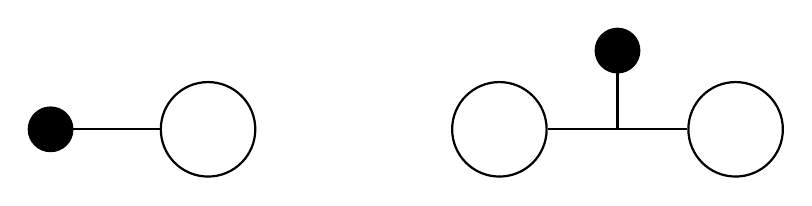
\begin{tikzpicture}[line width=0.9pt]

% ---------------------------
% 图1：s-channel
% ---------------------------
\begin{scope}[shift={(0,0)}]
 \node[source dot] (L) at (0, 0) {};
  \node[blob] (R) at ( 2.0,0.0) {};


  \begin{feynman}
    \vertex (M) at (1.0,0.0);
    
    \diagram*{
      (L) -- [draw=black, thick] (M),
      (M) -- [draw=black, thick] (R),
    };
  \end{feynman}


\end{scope}

% ---------------------------
% 图2：t-channel
% ---------------------------
\begin{scope}[shift={(7.2,0)}]
  \node[blob] (L) at (-1.5, 0) {};
  \node[blob] (R) at (1.5, 0) {};
  \node[source dot] (T) at (0, 1) {};

  \begin{feynman}
    \vertex (M) at (0.0,0.0);
    
    \diagram*{
      (L) -- [draw=black, thick] (M),
      (M) -- [draw=black, thick] (R),
      (T) -- [draw=black, thick] (M),
    };
  \end{feynman}
\end{scope}

%
\end{tikzpicture}



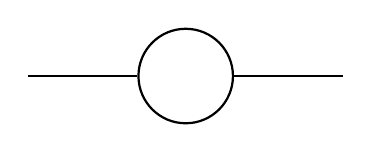
\begin{tikzpicture}
  \begin{feynman}
    \vertex (a) at (-2,0);
    \vertex[blob] (b) at (0,0) {};
    \vertex (c) at (2,0);

    \diagram*{
      (a) -- [plain] (b) -- [plain] (c),
    };
  \end{feynman}
\end{tikzpicture}



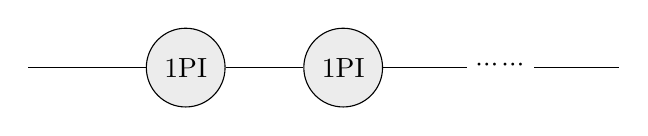
\begin{tikzpicture}
  \begin{feynman}
    \vertex (a) at (-2,0);
    \vertex[draw, circle, minimum size=1cm, fill=gray!15] (b) at (0,0) {1PI};
    \vertex[draw, circle, minimum size=1cm, fill=gray!15] (d) at (2,0) {1PI};
    \vertex[] (e) at (4,0) { $\cdots \cdots$};
    \vertex (f) at (5.5,0);

    \diagram*{
      (a) -- [plain] (b) --  [plain] (d) -- [plain] (e) -- [plain] (f),
    };
  \end{feynman}
\end{tikzpicture}


\end{document}